\documentclass{article}
\usepackage{hyperref}
\usepackage{listings}
\usepackage{color}
\usepackage{xcolor}
\usepackage{geometry}
\usepackage{graphicx}
\usepackage{amsmath}
\usepackage{caption}
\usepackage{subcaption}
\usepackage[capitalise]{cleveref}
\usepackage{wrapfig}
\usepackage{amssymb}

\geometry{margin=1in}
\pdfminorversion=6

\newcommand\TODO[1]{\textcolor{red}{TODO: #1}}

\newcommand\header[2]{
    \begin{center}
        {\large
        UCSD CSE 167 Assignment #1: \\
        \vspace{0.3cm}
        \Large
        #2}
    \end{center}
}

\definecolor{dkgreen}{rgb}{0,0.6,0}
\definecolor{gray}{rgb}{0.5,0.5,0.5}
\definecolor{mauve}{rgb}{0.58,0,0.82}
\lstset{frame=tb,
        aboveskip=3mm,
        belowskip=3mm,
        showstringspaces=false,
        columns=flexible,
        basicstyle={\small\ttfamily},
        numbers=none,
        numberstyle=\tiny\color{gray},
        keywordstyle=\color{blue},
        commentstyle=\color{dkgreen},
        stringstyle=\color{mauve},
        breaklines=true,
        breakatwhitespace=true,
        tabsize=2
}

% Taken from https://tex.stackexchange.com/questions/83085/how-to-improve-listings-display-of-json-files

\colorlet{punct}{red!60!black}
\definecolor{delim}{RGB}{20,105,176}
\colorlet{numb}{magenta!60!black}

\lstdefinelanguage{json}{
    basicstyle=\normalfont\ttfamily,
    numberstyle=\scriptsize,
    stepnumber=1,
    numbersep=8pt,
    showstringspaces=false,
    breaklines=true,
    frame=lines,
    tabsize=2,
    literate=
     *{0}{{{\color{numb}0}}}{1}
      {1}{{{\color{numb}1}}}{1}
      {2}{{{\color{numb}2}}}{1}
      {3}{{{\color{numb}3}}}{1}
      {4}{{{\color{numb}4}}}{1}
      {5}{{{\color{numb}5}}}{1}
      {6}{{{\color{numb}6}}}{1}
      {7}{{{\color{numb}7}}}{1}
      {8}{{{\color{numb}8}}}{1}
      {9}{{{\color{numb}9}}}{1}
      {:}{{{\color{punct}{:}}}}{1}
      {,}{{{\color{punct}{,}}}}{1}
      {\{}{{{\color{delim}{\{}}}}{1}
      {\}}{{{\color{delim}{\}}}}}{1}
      {[}{{{\color{delim}{[}}}}{1}
      {]}{{{\color{delim}{]}}}}{1},
}

\hypersetup{colorlinks=true}


\begin{document}

\header{1}{2D Graphics}
\setcounter{section}{-1}

\begin{figure}[ht]
    \centering
    \caption{Images we will produce in this homework.}
    \label{fig:teaser}
\end{figure}

Computer graphics is the field that studies how to process \emph{visual data}, such as shapes, volumes, and lights. \textbf{Images} are an important class of visual data: they can be the pictures recorded by the camera of your cellphone or a DSLR, outputs of video games or movie visual effects, legends and arrows on Google map telling you where to go next, or visualization of the radio waves coming from a black hole. An important subfield of computer graphics, rendering, studies the generation of images.

\begin{figure}[h]
    \centering
    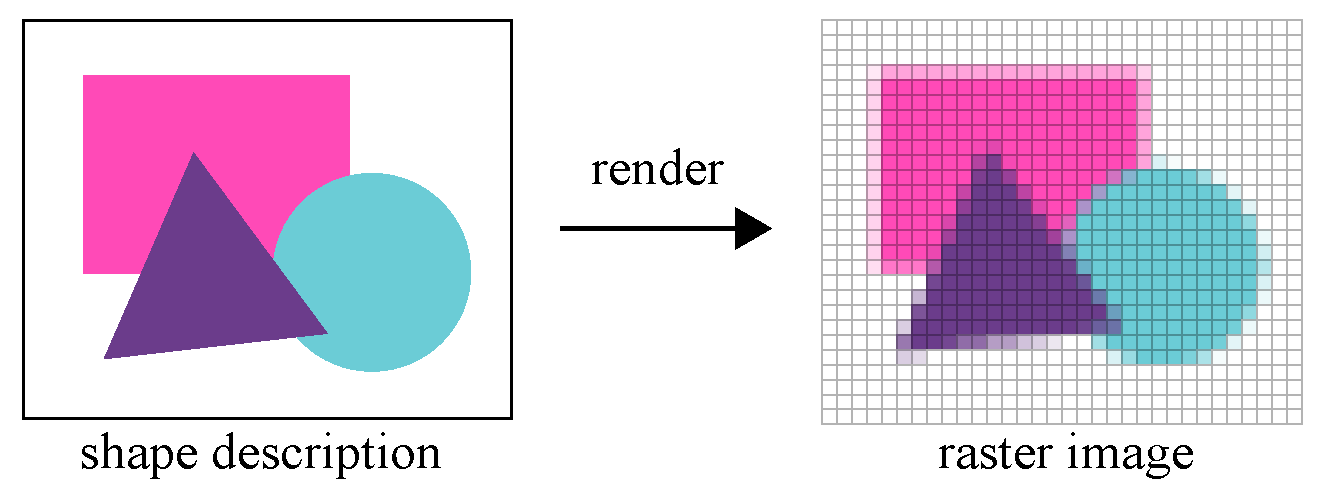
\includegraphics[width=0.6\linewidth]{imgs/render2d.pdf}
    \caption{In this homework, we will render a set of 2D shapes into a raster image.}
    \label{fig:render2d}
\end{figure}

In our first homework, we will implement a 2D renderer that takes a set of simple shapes (circle, squares, and triangles), and turn them into a raster image (\cref{fig:render2d}). A raster image is a particular kind of image that represent 2D contents using a grid of \emph{pixels}, where each pixel denotes the color at that location. Raster images are convienient because our displays (and our camera sensor) usually also represent images as a grid of pixels.

Before you start coding, we recommend you to go through the whole handout to have some ideas of what needs to be done.

\paragraph{Submission.} Submit your code and the outputs of your code through Canvas. In addition, for the quizzes below, answer them through the Gradescope (you can access it through Canvas).

\paragraph{Grading.} We will compare your outputs to our reference solutions. The points of the quizes are included in the total points on the section titles.

\paragraph{Colloboration policy.} We expect you to write the code on your own. Feel free to discuss between the peers and ask us questions though!

%\bibliographystyle{plain}
%\bibliography{refs}

\end{document}
